\section{物质波与粒子动量}

\subsection{从光子动量到德布罗意波长}

光子的能量、动量和真空波长满足
\[
 E=h\nu=\frac{hc}{\lambda},\qquad p=\frac Ec=\frac h\lambda.
\]
德布罗意把波长与动量的关系推广到有静质量的粒子：
\[
 \boxed{\lambda=\frac hp},\qquad p=\gamma mv.
\]
这里的波描述粒子出现的概率规律。电子衍射说明传播具有波动性，电子并非沿一条弯曲的正弦线运动。波长中的动量必须在指定参考系内求得；对有静质量的粒子，可承接相对论的能量动量关系，将 $E=K+mc^2$代入，依次得到
\[
 p^2c^2=(K+mc^2)^2-m^2c^4=K(K+2mc^2),
 \qquad \lambda=\frac{hc}{\sqrt{K(K+2mc^2)}}.
\]
当 $K\ll mc^2$时，根号中的 $K^2$可略，才恢复 $p\simeq\sqrt{2mK}=mv$。非相对论近似应检查动能与静能之比，不能只凭波长很短就判断速度大小。

同一动量对应同一德布罗意波长，并不要求质量或动能相同；同一动能的电子与质子则一般具有不同动量。对静电场加速，先由电势能减少求动能增加，再判断是否需要相对论动量，最后求波长。光子满足 $E=pc$，有静质量粒子不满足这一关系，两种能量代入方式不可互换。

\fig{fv:o7:diffraction}{不同路径的相位在同一探测点比较，波长不等于粒子的轨迹}{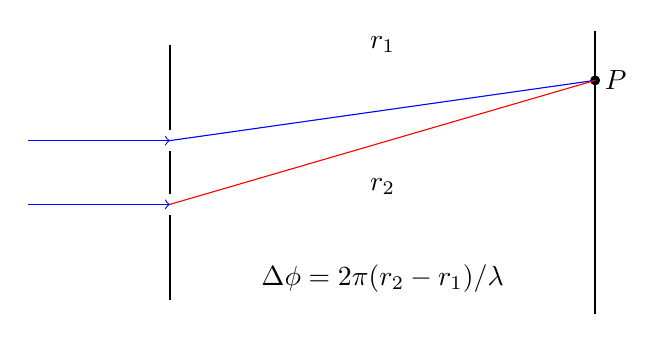
\begin{tikzpicture}[scale=.9]
\draw[thick](0,-1.8)--(0,-.6) (0,-.3)--(0,.3) (0,.6)--(0,1.8);
\draw[thick](6,-2)--(6,2);\fill(6,1.3)circle(2pt)node[right]{$P$};
\draw[->,blue](-2,.45)--(0,.45);\draw[->,blue](-2,-.45)--(0,-.45);
\draw[blue](0,.45)--(6,1.3);\draw[red](0,-.45)--(6,1.3);
\node at(3,1.8){$r_1$};\node at(3,-.2){$r_2$};\node at(3,-1.5){$\Delta\phi=2\pi(r_2-r_1)/\lambda$};
\end{tikzpicture}}
图\ref{fv:o7:diffraction}中的线段用来比较两条传播路径的相位，不能解释成电子同时沿两条确定的经典轨迹运动。动量确定空间相位的尺度 $\lambda=h/p$，到达 $P$的概率则由相应概率幅相加后取模平方得到。单个电子的探测是一个局域事件，多次重复才逐渐显示空间分布。若到达 $P$ 的两路概率幅分别为 $\psi_1(P),\psi_2(P)$，且没有区分路径的测量，则
\[
 \mathcal P(P)\propto|\psi_1+\psi_2|^2
 =|\psi_1|^2+|\psi_2|^2+2\operatorname{Re}(\psi_1^*\psi_2).
\]
图中的路程差进入最后一项的相位。被探测到的每个电子仍贡献一个局域记录；积累的空间分布检验的是这些记录的概率，不能把波长解释成单个电子在图中的上下摆动幅度。


\section{原子定态、类氢能级与谱线}

\subsection{玻尔模型：库仑力与角动量量子化}

先把氢核看作静止，电子质量为 \(m_e\)，电荷量大小为 \(e\)，记 \(k=1/(4\pi\varepsilon_0)\)，\(\hbar=h/(2\pi)\)。玻尔模型作如下假定：电子可处于若干不辐射的定态；圆轨道角动量满足
\[
 m_ev_nr_n=n\hbar,\qquad n=1,2,\ldots;
\]
定态间跃迁时才吸收或发射光子。圆轨道条件与量子化条件须同时满足。
\fig{fig:m3bohr}{半径、速度和库仑力的方向；圆轨道是玻尔模型中的图像}{
\begin{tikzpicture}[scale=1.05]
\draw[world] (0,0) circle(1.1);
\fill (0,0) circle(2pt) node[below left] {$O$（核）};
\fill (1.1,0) circle(2pt) node[right] {$A$（电子）};
\draw[dim] (0,-.25)--(1.1,-.25) node[midway,below] {$r_n$};
\draw[axis,thick] (1.1,0)--(1.1,.85) node[right] {$\bm v_n$};
\draw[axis,thick] (1.1,0)--(.25,0) node[midway,above] {$\bm F_C$};
\node[align=left] at (3.8,.35) {$F_C=ke^2/r_n^2$\\$m_ev_nr_n=n\hbar$};
\end{tikzpicture}}
图\ref{fig:m3bohr}中，\(A\) 点的库仑力沿 \(AO\) 向内，速度沿圆的切线。因此
\[
 \frac{ke^2}{r_n^2}=\frac{m_ev_n^2}{r_n},\qquad
 v_n=\frac{n\hbar}{m_er_n}.
\]
消去 \(v_n\)，再代回得
\[
 \boxed{r_n=n^2a_0},\quad a_0=\frac{\hbar^2}{m_eke^2}\approx5.29\times10^{-11}\,\mathrm m,
 \qquad v_n=\frac{ke^2}{n\hbar}.
\]
以无穷远为势能零点，径向向外取正，库仑力的径向分量为
$F_r=-ke^2/r^2$。由 $U(r)-U(\infty)=-\int_\infty^rF_r(s)\dd s$，
\[
 U(r)=ke^2\int_\infty^r s^{-2}\dd s
 =ke^2[-s^{-1}]_\infty^r=-\frac{ke^2}{r}.
\]
再由圆周运动方程乘以 $r_n/2$ 得
\(K_n=m_ev_n^2/2=ke^2/(2r_n)\)。将动能与势能相加，故
\[
 \boxed{E_n=-\frac{ke^2}{2r_n}=-\frac{m_ek^2e^4}{2n^2\hbar^2}
       =-\frac{E_B}{n^2}},\qquad E_B\approx13.6\,\mathrm{eV}.
\]
负号表示束缚态；电离能为 \(-E_n=E_B/n^2\)。第一激发态是 \(n=2\)，其激发能为 \(E_2-E_1=3E_B/4\)，不是 \(|E_2|\)。

\fig{o7:phase-closure}{将玻尔圆轨道的周长展开，检查绕行一周的相位闭合；波线表示相位的周期}{\begin{tikzpicture}

\draw[world](0,0)circle(1);\fill(0,0)circle(1.5pt)node[left]{核};
\draw[axis](1,0)--(1,.7)node[right]{$p$};
\draw[dim](0,-.25)--(1,-.25)node[midway,below]{$r_n$};
\draw[axis](1.45,-.3)--(2.3,-.3);
\begin{scope}[xshift=3cm,yshift=-.3cm,x=.8cm]
\draw[axis](0,0)--(6.5,0)node[right]{$s$};
\draw[blue,thick,domain=0:6,samples=180]plot(\x,{.4*sin(180*\x)});
\draw[dim](0,-.75)--(6,-.75)node[midway,below]{$2\pi r_n=n\lambda$};
\draw[dim](0,.75)--(2,.75)node[midway,above]{$\lambda$};
\node[above]at(3,1.3){图示 $n=3$};
\end{scope}

\end{tikzpicture}}

图\ref{o7:phase-closure}中，绕行一周须使相位增加 $2\pi n$。圆周上容纳整数个波长的条件 $2\pi r_n=n\lambda$，结合 \(\lambda=h/(m_ev_n)\)，也得到角动量量子化。这是对玻尔圆轨道条件的直观解释。实际原子中的定态由波函数描述，圆轨道并不是电子真实路径的完整描述。

\subsection{核电荷数与类氢能级}
先把库仑力中的核电荷数 \(Z\) 写清楚，再使用角动量量子化。忽略核运动时，
\[
 \frac{kZe^2}{r_n^2}=\frac{m_ev_n^2}{r_n},\qquad
 m_ev_nr_n=n\hbar.
\]
联立得到
\[
 r_n=\frac{n^2}{Z}a_0,\qquad v_n=\frac Zn v_0,\qquad
 E_n=-13.6\,\frac{Z^2}{n^2}\,\mathrm{eV}.
\]
这里 \(a_0=5.29\times10^{-11}\,\mathrm m\)，\(v_0=2.19\times10^6\,\mathrm{m/s}\)。这些关系采用固定核近似；有限核质量需要以约化质量替换电子质量。

\fig{o7:z-energy-scale}{相同电子量子数下，单电子氦离子的束缚能为氢的四倍；同一能量比例示意}{\begin{tikzpicture}

\begin{scope}[y=.055cm]
\draw[axis](-.7,-59)--(-.7,10)node[above]{$E/\mathrm{eV}$};
\draw[world](0,0)--(2,0) (0,-3.4)--(2,-3.4) (0,-13.6)--(2,-13.6);
\draw[world](4.7,0)--(6.7,0) (4.7,-13.6)--(6.7,-13.6) (4.7,-54.4)--(6.7,-54.4);
\node[above]at(1,10){氢 $Z=1$};\node[above]at(5.7,10){$\mathrm{He}^+$，$Z=2$};
\node[left]at(-.7,0){$0$};\node[left]at(-.7,-13.6){$-13.6$};\node[left]at(-.7,-54.4){$-54.4$};
\node[right]at(2,-3.4){$n=2$};\node[right]at(2,-13.6){$n=1$};
\node[right]at(6.7,-13.6){$n=2$};\node[right]at(6.7,-54.4){$n=1$};
\end{scope}

\end{tikzpicture}}
图\ref{o7:z-energy-scale}中，$Z$ 加倍使同一 $n$ 的半径减半、轨道速率加倍，动能和束缚能的尺度均增为四倍。这里只讨论单电子库仑体系；中性氦有两个电子，电子间相互作用使这些类氢公式不能直接套用。还应检查 $v_n/c=(Z/n)v_0/c\ll1$，否则玻尔模型的非相对论近似不足。

\subsection{能级图与谱线}

\fig{fig:m3levels}{能级越高，间隔越密；图中纵向间距作了示意性放大}{
\begin{tikzpicture}[x=1cm,y=1cm]
\draw[axis] (-.3,-.2)--(-.3,3.7) node[above] {$E$};
\foreach \y/\n/\e in {0/1/{-13.6},2/2/{-3.40},2.8/3/{-1.51},3.2/4/{-0.85}}{
\draw[world] (.1,\y)--(4.9,\y);\node[right] at(4.9,\y){$n=\n$};\node[left] at(-.35,\y){$\e$};}
\draw[aux] (.1,3.6)--(4.9,3.6) node[right] {$n\to\infty$};
\node[left] at(-.35,3.6){$0$};
\draw[axis,thick] (1,2.8)--(1,2) node[midway,left] {$H_\alpha$};
\draw[axis,thick] (2.6,2)--(2.6,0) node[midway,right] {$\Delta_{21}$};
\draw[axis,thick] (4,0)--(4,2.8) node[midway,right] {$\Delta_{31}$};
\node at(2.3,-.55){能量单位：\(\mathrm{eV}\)};
\end{tikzpicture}}
图\ref{fig:m3levels}中，向下箭头对应发射，向上箭头对应吸收。忽略原子整体反冲时，\(n_i\to n_f\) 的光子满足
\[
 h\nu=|E_{n_i}-E_{n_f}|,\qquad
 \frac1\lambda=R_H\left|\frac1{n_f^2}-\frac1{n_i^2}\right|,
 \quad R_H=\frac{E_B}{hc}.
\]
终态 \(n_f=1,2,3\) 分别构成莱曼系、巴耳末系、帕邢系。巴耳末系首线 \(H_\alpha\) 是 \(3\to2\)，不能把它与 \(2\to1\) 的跃迁混淆。处于 \(n=3\) 的原子既可直接回到 \(n=1\)，也可先到 \(n=2\)；后一条级联路径才能发出 \(H_\alpha\)。

图\ref{fig:m3levels}的纵轴表示整个原子内部的总能量，不能把箭头长度解释成电子动能的变化。定态中库仑势能与动能会同时改变，二者之和才决定跃迁能量。能级的零点选在电离极限，所以从 $n$ 态电离只需增加 $E_B/n^2$，并不是增加 $E_B$。

对固定终态的谱线系列，初态越高，发射光子能量越大，波长越短；当初态趋于无穷远时达到该系列的短波极限。初态固定时，一次原子衰变只能沿某条直接或级联路径下降，不能在同一次衰变中任意发出所有可能能级差。大量原子的不同衰变路径叠加后，才可能观察到多条谱线。数谱线或判断是否出现某条谱线时，应先说明讨论的是单个原子的一次过程，还是原子集合的统计结果。

\section{有限核质量与跃迁反冲}

\subsection{有限核质量：内部运动与整体运动}

以下先取氢原子 $Z=1$。核质量为 $M_N$ 时，电子和核都绕质心运动。令相对坐标 \(\bm r=\bm r_e-\bm r_N\)，约化质量为
\[
 \mu=\frac{m_eM_N}{m_e+M_N}.
\]
内部相对运动满足 \(\mu v_{\rm rel}r=n\hbar\) 与 \(ke^2/r^2=\mu v_{\rm rel}^2/r\)，所以上述公式中的 \(m_e\) 应替换为 \(\mu\)：
\[
 r_n=\frac{n^2\hbar^2}{\mu ke^2},\quad
 E_n=-\frac{\mu k^2e^4}{2n^2\hbar^2},\quad
 \boxed{R_M=R_\infty\frac{\mu}{m_e}=\frac{R_\infty}{1+m_e/M_N}}.
\]
这里的 \(r_n\) 是电子与核的间距。有限核质量改变的是内部能级；跃迁时原子质心获得动量，则属于整体反冲，两种效应须分别计算。

\fig{fig:m3relative-coordinate}{电子和核到质心的距离不同，间距之和为相对坐标长度}{\begin{tikzpicture}
\draw[axisline](-.8,0)--(6.1,0);
\fill(0,0)circle(3pt)node[above]{$M_N$};
\fill(1.2,0)circle(1.5pt)node[above]{$C$};
\fill(5,0)circle(2pt)node[above]{$m_e$};
\draw[dim](0,-.5)--(1.2,-.5)node[midway,below]{$r_N$};
\draw[dim](1.2,-.5)--(5,-.5)node[midway,below]{$r_e$};
\draw[dim](0,-1.2)--(5,-1.2)node[midway,below]{$r$};
\node at(2.5,1){$M_Nr_N=m_er_e$};
\end{tikzpicture}}
图\ref{fig:m3relative-coordinate}示意质心分配关系；为显示核的运动，距离不按真实比例绘制。由 $M_Nr_N=m_er_e$ 与 $r=r_N+r_e$，得
$r_e=M_Nr/(M_N+m_e)$、$r_N=m_er/(M_N+m_e)$。二者同角速度转动，设角速度为 $\omega$，两部分动能之和为
\[
 T_{\rm int}=\frac12m_e\omega^2r_e^2+\frac12M_N\omega^2r_N^2
 =\frac12\frac{m_eM_N}{m_e+M_N}\omega^2r^2
 =\frac12\mu v_{\rm rel}^2.
\]
因此内部运动的惯量由约化质量承担。对一般核电荷数 $Z$，还应把库仑因子 $ke^2$ 换成 $kZe^2$，能级相应含 $Z^2$。

当 $M_N\to\infty$，质心趋向核，$\mu\to m_e$，恢复固定核近似；有限核质量使 $\mu<m_e$，能级结合能的绝对值略减小，波长相应改变。这种改变在跃迁之前就已包含在内部能级中，不能再把同一效应重复算成发射光子的整体反冲。

\subsection{跃迁能对应静质量差}

设基态原子静质量为 \(m_0\)，某激发态高出能量 \(\Delta\)，则激发态的静质量为
\[
 \boxed{m_*=m_0+\frac{\Delta}{c^2}}.
\]
\(\Delta\) 是两个静止原子内部能量之差。自由原子发射光子时要分出反冲动能，故光子能量小于 \(\Delta\)；静止基态原子吸收一个光子后会整体运动，入射光子能量须大于 \(\Delta\)。例\ref{ex:m3recoil}将用能量和动量守恒求出这两个差值。

静质量包含体系在自身质心系中的全部内部能量，因此原子受激后即使整体仍静止，质量也比基态大。这里增加的是原子整体的静质量，不能只给电子的质量单独加上 $\Delta/c^2$，同时又把电子轨道能完整保留一次。

\fig{o7:emission-absorption}{自由原子的发射与吸收均需给整体动量；两幅图分别从各自初态静止的条件出发}{\begin{tikzpicture}

\begin{scope}
\node[above]at(1.7,1.4){发射：初态 $m_*$ 静止};
\fill(1.7,0)circle(2.5pt)node[below]{$m_0$};
\draw[axis,thick](1.6,.5)--(.1,.5)node[midway,above]{反冲};
\draw[ray,red](1.8,0)--(3.9,0)node[right]{$E_{\rm em}$};
\node[below]at(1.7,-.8){$\Delta=E_{\rm em}+K_{\rm rec}$};
\end{scope}
\begin{scope}[xshift=6.5cm]
\node[above]at(1.7,1.4){吸收：初态 $m_0$ 静止};
\draw[ray,red](-.3,0)--(1.6,0)node[midway,above]{$E_{\rm abs}$};
\fill(1.7,0)circle(2.5pt)node[below]{$m_*$};
\draw[axis,thick](1.8,.5)--(3.3,.5)node[midway,above]{整体运动};
\node[below]at(1.7,-.8){$E_{\rm abs}=\Delta+K_{\rm rec}$};
\end{scope}

\end{tikzpicture}}
图\ref{o7:emission-absorption}把质心反冲与内部状态分开画出。发射时，光子向右而末态原子向左；吸收时，入射光子消失，其动量由末态原子向右运动承担。$m_0$ 与 $m_*$ 是原子不同内部状态的静质量，箭头表示整体运动。

若初态激发原子静止，自由发射后动量守恒要求原子反冲，故
$\Delta=E_\gamma+K_{\rm rec}$。在反冲非相对论时，
$K_{\rm rec}\simeq E_\gamma^2/(2m_0c^2)$，因此光子能量略低于内部能级差。吸收时同样须给末态原子动量，关系改为 $E_\gamma=\Delta+K_{\rm rec}$，所以所需光子能量略高。两种偏差的符号由动能必须非负直接决定，是检查精确公式的可靠方法。

\section{碰撞激发与能量分配}

\subsection{质心平动能与内部相对运动能}
碰撞前后系统总动量守恒。实验室中的整体平动能不能随意消失，能用于内部激发的是相对运动能。对两粒子，
\[
 K_{\rm tot}=\frac12(m+M)V_{\rm cm}^2+
 \frac12\mu v_{\rm rel}^2,\qquad \mu=\frac{mM}{m+M}.
\]
建立方程时应分别标出质量、实验室速度和质心速度，再比较内部能级差。

\fig{o7:collision-energy}{静止靶碰撞的两种参考系；阈值末态在质心系没有相对运动}{\begin{tikzpicture}

\node[left]at(0,1.3){实验室初态};
\fill(1,1.3)circle(2.5pt)node[below]{$m$};\fill(5,1.3)circle(3pt)node[below]{$M$};
\draw[axis](1,1.9)--(3,1.9)node[midway,above]{$v$};\node[above]at(5,1.6){静止};
\node[left]at(0,-.5){质心系初态};
\fill(1,-.5)circle(2.5pt)node[below]{$m$};\fill(5,-.5)circle(3pt)node[below]{$M$};
\draw[axis](1,.1)--(2.9,.1)node[midway,above]{$v-V_{\rm cm}$};
\draw[axis](5,.1)--(3.8,.1)node[midway,above]{$-V_{\rm cm}$};
\node[below,align=center]at(3,-1.6){阈值末态：质心系中两者均静止\\相对运动能恰好全部用于内部激发};

\end{tikzpicture}}
图\ref{o7:collision-energy}中，初态 $V_{\rm cm}=mv/(m+M)$。在质心系，两个动量等值反向，故内部可用动能为
\[
 \frac12m(v-V_{\rm cm})^2+\frac12MV_{\rm cm}^2
 =\frac12\mu v^2.
\]
回到实验室时还须加上 $\tfrac12(m+M)V_{\rm cm}^2$。这项由总动量决定，封闭系统内的碰撞不能把它任意转成激发能。

\subsection{能级差、光子能量与碰撞阈能}

图\ref{fig:m3levels}上的两条水平线之差是原子内部能量差 $\Delta$。图中的箭头只说明内部状态改变，不表示所有激发方式都只需提供大小为 $\Delta$ 的入射动能。是否还需要给原子整体动量，必须由具体过程决定。

跃迁反冲的讨论已经由反冲动能非负判断了自由发射和吸收的能量偏移。若外部支撑能承担动量、且其能量变化可忽略，才可把光子能量近似等同于 $\Delta$。下面改为粒子碰撞：其入射动量由两物体共同承担，须先分离不能转入激发的质心动能。

粒子碰撞则可能在激发后仍有剩余动能。对质量 $m$ 的入射粒子撞击静止质量 $M$ 的原子，先在非相对论、忽略激发引起质量微小变化的模型下分解初动能：
\[
 K_{\text{入}}=K_{\text{质心}}+K_{\text{相对}},\qquad
 K_{\text{相对}}=\frac{M}{m+M}K_{\text{入}}.
\]
总动量守恒要求质心运动不能任意消失，真正能转入内部激发的是相对运动能。阈值处末态相对运动能恰好为零，故
\[
 K_{\text{相对}}\ge\Delta,\qquad
 \boxed{K_{\text{入,阈}}=\left(1+\frac mM\right)\Delta}.
\]
入射电子远轻于原子时，阈能近似为 $\Delta$；入射粒子与原子等质量时，阈能近似为 $2\Delta$。激发是否允许还不等于每次碰撞都会发生激发。图\ref{o7:collision-energy}的阈值末态在实验室中仍以 $V_{\rm cm}$ 共同平移。实际使用时须检查原子的初始运动和碰撞几何，并保证所用非相对论近似成立。

本讲数值计算取 \(h=6.626\times10^{-34}\,\mathrm{J\,s}\)，\(c=2.998\times10^8\,\mathrm{m/s}\)，\(e=1.602\times10^{-19}\,\mathrm C\)，\(m_ec^2=0.511\,\mathrm{MeV}\)。氢原子能级取 \(E_B=13.6\,\mathrm{eV}\) 时只保留相应精度；精细结构和辐射修正不在本讲模型内。
